\begin{figure}[H]
	\centering
	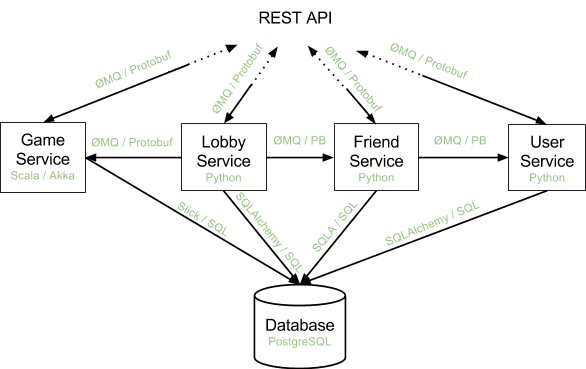
\includegraphics[width=\textwidth,height=\textheight,keepaspectratio=true]{img/sPVjzeXSLniaBJWqfNTsV4A.png}
	\caption{The infrastructure of the server backend. Each arrow indicates communication between respective services and green text indicates the main technologies used for the various entities.}
	\label{fig:sysarch}
\end{figure}

\subsection{Backend}
The backend is divided into smaller parts and composed as services that run as independent processes, where each service handles a distinct part of the business logic. To enable services to talk between each other, ZeroMQ is used as the transport layer and Protocol Buffers is employed as the serialization or transport format to enable different languages to share the same protocol. ZeroMQ readily allows for implementation of message patterns such as the request/reply model and the publish/subscribe paradigm, and we have used the former pattern for the primary communication between processes and the latter pattern for websocket push notifications.
An easily extendable architecture for the Python processes is built based on an inheritable base class that together with a shared protocol structure allows for quick development of new services. The architecture also allows for expedient definition of new methods that are callable by RPC messaging via ZeroMQ and Protocol Buffers. 

\subsubsection{Game Service}
Built with scalability in mind, the game process handles all the game logic in individual games, as well as the creation and maintenance of new games, and the pruning of old games. Internally, the game utilizes a load broker pattern for load balancing to allow many ZeroMQ requests to be handled simultaneously, and uses Akka to parallelize the requests. The Slick API is used throughout to save game state to the database.

\subsubsection{Lobby Service}
This is a service that handles the creation of games. This service has functionality to create a lobby, remove a lobby and start a game. When a user has created a lobby the user can send invitations to friends and the friends can accept or deny these invitations. This service is used when a user checks which lobbies said user is a member of. 

\subsubsection{User Service}
This service handles the users of the system. The service has functionality to authenticate, create and get users. The service is used when a user is created and when a user logs in. When a user tries to add another user as a friend this service is used to make sure that the provided email address for the friend really exists. 

\subsubsection{Friends Service}
This is a service that handles the users connection with friends. The service gives the functionality to add a friend, remove a friend or to list all friends. The service is used when a user manages the friends list. It is also used while creating a game. The user can choose friends from the current friends list whom the user wishes to play with and invite them to a game lobby.

\subsection{Web/RESTful API}
As can be seen in Figure \ref{fig:sysarch} the REST API is in the top and can call the different services with protocol buffers messages over ZMQ. The Web application Flask server is just like the REST API located in the top and use the services in the same manner as the REST API.

\subsection{Mobile Clients}
The mobile clients communicate with the backend using the web api, this communication is made using simple http-requests to different urls with custom headers such as user-token and sometimes providing data using a body of json. The responses are either just a verification that the request was made successfully or a body of json with information. Creating and handling these requests and responses in each and every view directly would be tedious and unnecessary so the focus and most work for each client has been creating a communication manager that handles these requests as easily as possible. We wanted these communication managers to be made in such a way that you could easily expand upon them when new features are added to the backend. The android and iOS client has each achieved this in a different way but achieved it nonetheless. 